\documentclass{article}
\usepackage{tikz}
\usetikzlibrary{arrows}
\begin{document}
	\title{Test Problem2}
	\author{Rashi}
	\date{\today}
	\maketitle
	In a mathematician’s terminology, a graph is a collection of points and lines
	connecting some (possibly empty) subset of them. The points of a graph are
	most commonly known as graph vertices, but may also be called ”nodes” or
	simply ”points.” Similarly, the lines connecting the vertices of a graph are most
	commonly known as graph edges, but may also be called ”arcs” or ”lines.”\\
	
	
	\begin{tikzpicture}
	[scale=.6,auto=center]
	\tikzset{edge/.style = {->,> = latex'}}
	\node (n1) at (0,0) {1}; 
	\node (n2) at (6,-7) {2};
	\node (n3) at (15,-7) {3};
	
	\foreach \from/\to in {n1/n2,n2/n3}
	\draw (\from)--(\to);
	\end{tikzpicture}
	\begin{center}Figure 1: Simple graph with three nodes
	\end{center}
\vspace{0.7cm}
The study of graphs is known as graph theory, and was first systematically
investigated by D. Knig in the 1930s (Gardner 1984, p. 91). Unfortunately,
as Gardner (1984, p. 91) notes, ”The confusion of this term [i.e., the term
”graph” to describe a network of vertices and edges] with the ’graphs’ of analytic
geometry [i.e., plots of functions] is regrettable, but the term has stuck.” Some
educators use the term ”vertex-edge graph” for a connected set of nodes in
an attempt to preserve the common usage of ”graph” to mean the plot of a
function.\\
\begin{tikzpicture}

\tikzset{vertex/.style = {shape=circle,fill=brown,draw,minimum size=1.5em}}
\tikzset{vertex2/.style = {shape=rectangle,fill=green}} 
\tikzset{edge/.style = {->,> = latex'}}
% vertices
\node[vertex2] (4) at  (0,0) {4};
\node[vertex2] (3) at  (11.5,0) {3};
\node[vertex2] (1) at  (0,-11.5) {1};
\node[vertex2] (2) at  (11.5,-11.5) {2};
%edges
\draw[edge] (1) to (2);
\draw[edge] (2) to (3);
\draw[edge] (3) to (4);
\draw[edge] (4) to (1);
\draw[edge] (3) to (1);
\end{tikzpicture}
\begin{center}Figure 2: Directed graph with four nodes
\end{center}
The study of graphs is known as graph theory, and was first systematically in-
vestigated by D. Knig in the 1930s (Gardner 1984, p. 91). Unfortunately, as
Gardner (1984, p. 91) notes, ”The confusion of this term [i.e., the term ”graph”
to describe a network of vertices and edges] with the ’graphs’ of analytic ge-
ometry [i.e., plots of functions] is regrettable, but the term has stuck.” Someeducators use the term ”vertex-edge graph” for a connected set of nodes in an
attempt to preserve the common usage of ”graph” to mean the plot of a func-\\

tion.The study of graphs is known as graph theory, and was first systematically
investigated by D. Knig in the 1930s (Gardner 1984, p. 91). Unfortunately,
as Gardner (1984, p. 91) notes, ”The confusion of this term [i.e., the term
”graph” to describe a network of vertices and edges] with the ’graphs’ of ana-
lytic geometry [i.e., plots of functions] is regrettable, but the term has stuck.”
Some educators use the term ”vertex-edge graph” for a connected set of nodes
in an attempt to preserve the common usage of ”graph” to mean the plot of a
function.\\
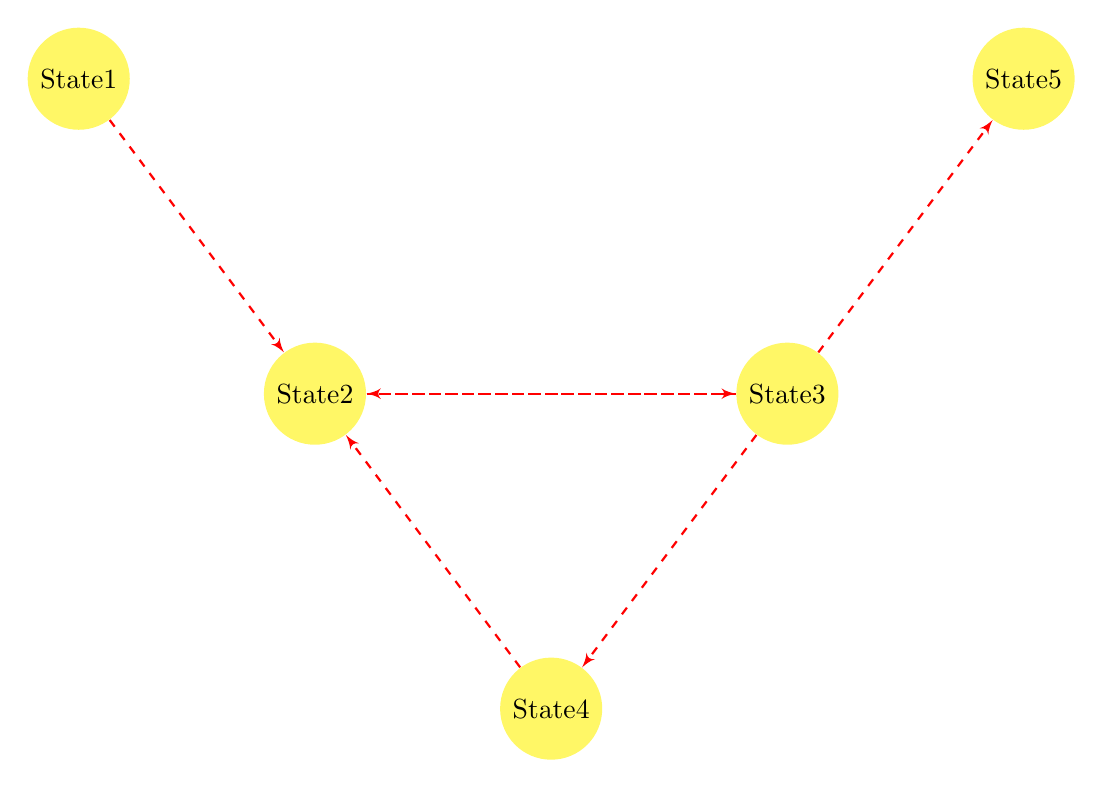
\begin{tikzpicture}

\tikzset{vertex/.style = {shape=circle,fill=yellow!60,minimum size=3em}}
\tikzset{vertex2/.style = {shape=rectangle,fill=green}} 
\tikzset{edge/.style = {->,> = latex',dashed,red,thick}}
%\tikzset{edge/.style = {<->,> = latex'}}
% vertices
\node[vertex] (State1) at  (0,0) {State1};
\node[vertex] (State5) at  (12,0) {State5};
\node[vertex] (State4) at  (6,-8) {State4};
\node[vertex] (State2) at  (3,-4) {State2};
\node[vertex] (State3) at  (9,-4) {State3};
%edges
\draw[edge] (State1) to (State2);
\draw[edge] (State2) to (State3);
\draw[edge] (State3) to (State2);
\draw[edge] (State4) to (State2);
\draw[edge] (State3) to (State5);
\draw[edge] (State3) to (State4);
\end{tikzpicture}
\begin{center}Figure 3: Directed graph with 5 nodes
\end{center}
The study of graphs is known as graph theory, and was first systematically
investigated by D. Knig in the 1930s (Gardner 1984, p. 91). Unfortunately,
as Gardner (1984, p. 91) notes, ”The confusion of this term [i.e., the term
”graph” to describe a network of vertices and edges] with the ’graphs’ of analytic
geometry [i.e., plots of functions] is regrettable, but the term has stuck.” Some
educators use the term ”vertex-edge graph” for a connected set of nodes in an
attempt to preserve the common usage of ”graph” to mean the plot of a function.


\end{document}